\documentclass[aspectratio=169,xcolor=dvipsnames]{beamer}
\usetheme{SimplePlus}

\usepackage{hyperref}
\usepackage{graphicx} % Allows including images
\usepackage{booktabs} % Allows the use of \toprule, \midrule and \bottomrule in tables

\title{Nobel Ontology}
\subtitle{Group A3D}

\author{Andrea Bruttomesso, Alessandro Corr\`o, Davide Seghetto, Andrea Stocco}

\date{\today} % Date, can be changed to a custom date

\setbeamertemplate{footline}{\leavevmode%
\begin{beamercolorbox}[wd=.33\paperwidth,left,ht=2.5ex,dp=1.5ex,leftskip=0.5ex]{subsection in head/foot} A3D
\end{beamercolorbox}%
\begin{beamercolorbox}[wd=.33\paperwidth,center,ht=2.5ex,dp=1.5ex]{section in head/foot}
  \usebeamercolor[fg]{section in foot/head}\insertshorttitle
\end{beamercolorbox}%
\begin{beamercolorbox}[wd=.34\paperwidth,right,ht=2.5ex,dp=1.5ex, rightskip=1.5ex]{subsection in head/foot}
  \insertshortdate
\end{beamercolorbox}%
}

%----------------------------------------------------------------------------------------
%    PRESENTATION SLIDES
%----------------------------------------------------------------------------------------
\begin{document}

\begin{frame}
	% Print the title page as the first slide
	\titlepage
\end{frame}

\begin{frame}{Overview}
	% Throughout your presentation, if you choose to use \section{} and \subsection{} commands, these will automatically be printed on this slide as an overview of your presentation
	\tableofcontents
\end{frame}

\section{Domain of Interest}

\begin{frame}{Domain of Interest}
	\centering
	\begin{minipage}{0.3\textwidth}
		\centering
		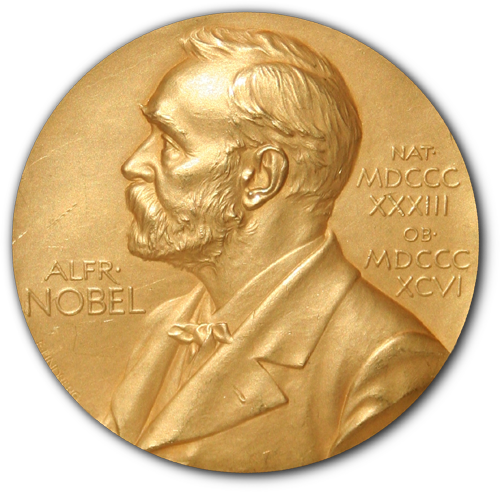
\includegraphics[width=\textwidth]{nobel.png} % Left image
	\end{minipage}%
	\hspace{3em}
	\begin{minipage}{0.4\textwidth}
		\centering
		We have chosen the domain of scientific research. Specifically, we aim to analyze potential correlations among Nobel Prize winners,
		their publications, and the research funding invested by various countries. This domain was selected because it allows us to reveal potential historical
		and geographical patterns in scientific research.
	\end{minipage}%
\end{frame}

\section{Ontology Design}

\begin{frame}{Nobel Ontology}
	\begin{figure}
		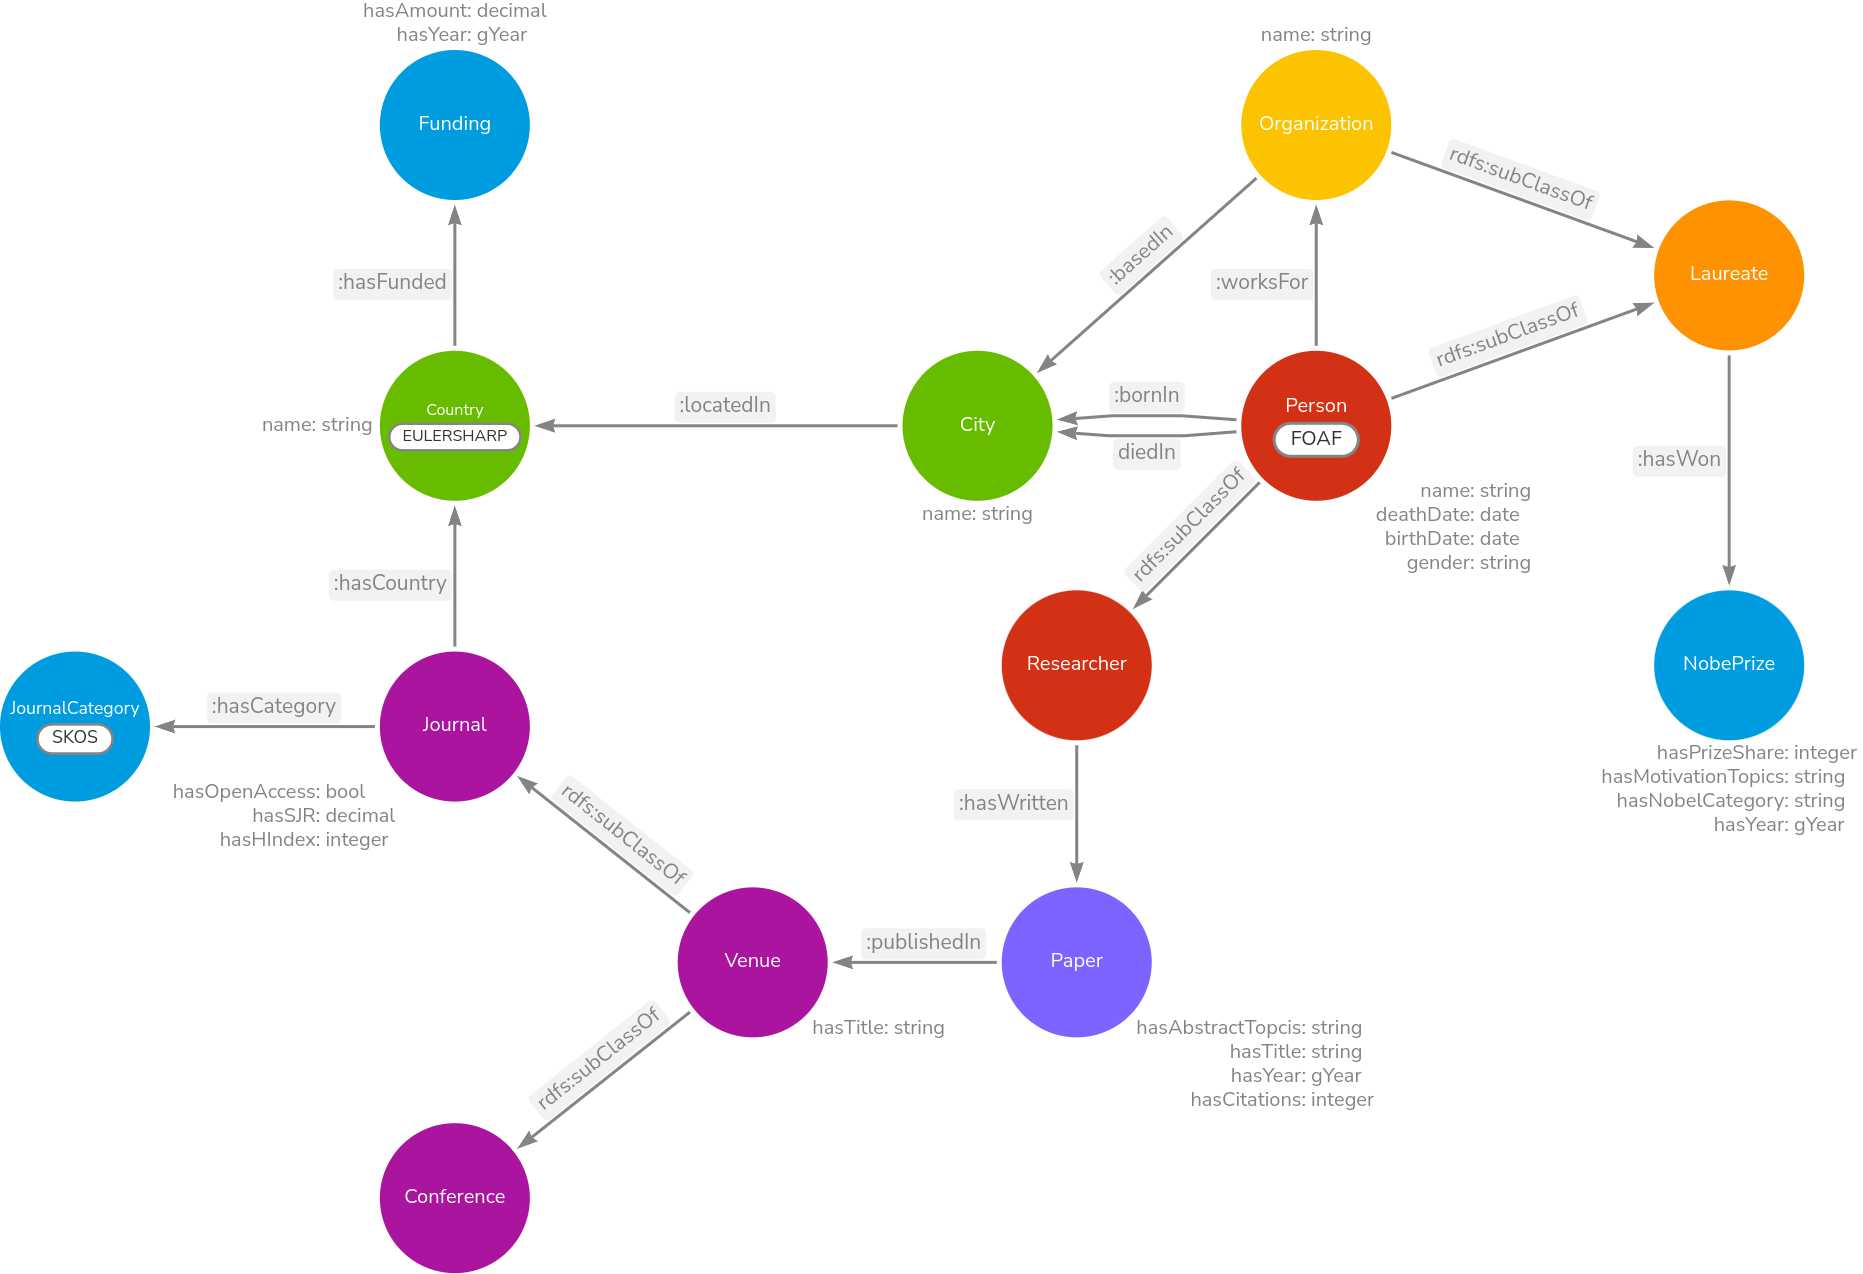
\includegraphics[width=0.75\linewidth]{../nobelOntologyTransparent.png}
	\end{figure}
\end{frame}

\section{Problems}

\begin{frame}{Problems}
	\begin{itemize}
		\item Errors in Nobel laureates dataset
		\item Subset of papers dataset
		\item Researchers and Nobel laureates matching
	\end{itemize}
\end{frame}

\begin{frame}{Errors in Nobel-Laureate dataset}
	\begin{table}[H]
		\centering
		\caption{Example of dataset error}
		\resizebox{.6\linewidth}{!}{\begin{tabular}{|l|l|l|l|}
				\hline
				\textbf{Year} & \textbf{Category} & \textbf{Prize Share} & \textbf{Full Name}    \\ \hline
				1908          & Medicine          & 1/2                  & Ilya Ilyich Mechnikov \\ \hline
				1908          & Medicine          & 1/2                  & Paul Ehrlich          \\ \hline
				1908          & Medicine          & 1/2                  & Paul Ehrlich          \\ \hline
			\end{tabular}}
		\label{tab:datasetError}
	\end{table}
\end{frame}

\section{Analytics}

\begin{frame}{Relationship between Nobel Prize winning ideas and published studies}
	\begin{columns}[c]
		\column{0.45\textwidth}
		\begin{table}[H]
			\centering
			\caption{Number of papers per Nobel topic in 2004}
			\resizebox{\linewidth}{!}{\begin{tabular}{|l|l|c|}
					\hline
					\textbf{Nobel topic} & \textbf{Nobel Prize} & \textbf{Number of papers} \\ \hline
					protein              & Chemistry 2004       & 28                        \\ \hline
					development          & Peace 2004           & 13                        \\ \hline
					flow                 & Literature 2004      & 8                         \\ \hline
					interaction          & Physics 2004         & 4                         \\ \hline
					discovery            & Chemistry 2004       & 3                         \\ \hline
					discovery            & Physics 2004         & 3                         \\ \hline
					degradation          & Chemistry 2004       & 3                         \\ \hline
					asymptotic           & Physics 2004         & 2                         \\ \hline
					forces               & Economics 2004       & 1                         \\ \hline
					cycles               & Economics 2004       & 1                         \\ \hline
					olfactory            & Medicine 2004        & 1                         \\ \hline
					organization         & Medicine 2004        & 1                         \\ \hline
				\end{tabular}}
			\label{tab:papersNobelTopicsYear}
		\end{table}
		\column{.45\textwidth}
		The topic ``protein'' appeared in 28 papers. The high number of papers mentioning this Nobel topic suggests that
		it was widely discussed or relevant in 2004.
	\end{columns}
\end{frame}

\begin{frame}{Most active research areas in a year}
	\begin{columns}
		\column{.45\textwidth}
		\begin{table}[H]
			\centering
			\caption{Number of papers for each journal subcategory in 2004}
			\resizebox{\linewidth}{!}{\begin{tabular}{|l|c|}
					\hline
					\textbf{Journal Subcategory}            & \textbf{Number of papers} \\ \hline
					Biochemistry Genetics Molecular Biology & 418                       \\ \hline
					Social Sciences                         & 344                       \\ \hline
					Decision Sciences                       & 125                       \\ \hline
					Arts Humanities                         & 74                        \\ \hline
					Business Management Accounting          & 68                        \\ \hline
					Physics Astronomy                       & 65                        \\ \hline
					Neuroscience                            & 55                        \\ \hline
					Health Professions                      & 34                        \\ \hline
					Psychology                              & 27                        \\ \hline
					Earth Planetary Sciences                & 22                        \\ \hline
					Economics Econometrics Finance          & 14                        \\ \hline
					Materials Science                       & 12                        \\ \hline
					Environmental Science                   & 12                        \\ \hline
					Agricultural Biological Sciences        & 10                        \\ \hline
					Energy                                  & 2                         \\ \hline
					Pharmacology Toxicology Pharmaceutics   & 2                         \\ \hline
				\end{tabular}}
			\label{tab:papersPerSubcategoryPerYear}
		\end{table}
		\column{.45\textwidth}
		Molecular biology was the most active research area in 2004.\\
	\end{columns}
\end{frame}

\begin{frame}
	\Huge{\centerline{\textbf{Questions?}}}
\end{frame}

\end{document}
